%! Author = paulsenik
%! Date = 12.09.23

\begin{frame}{Die Konsole}
    \begin{center}
        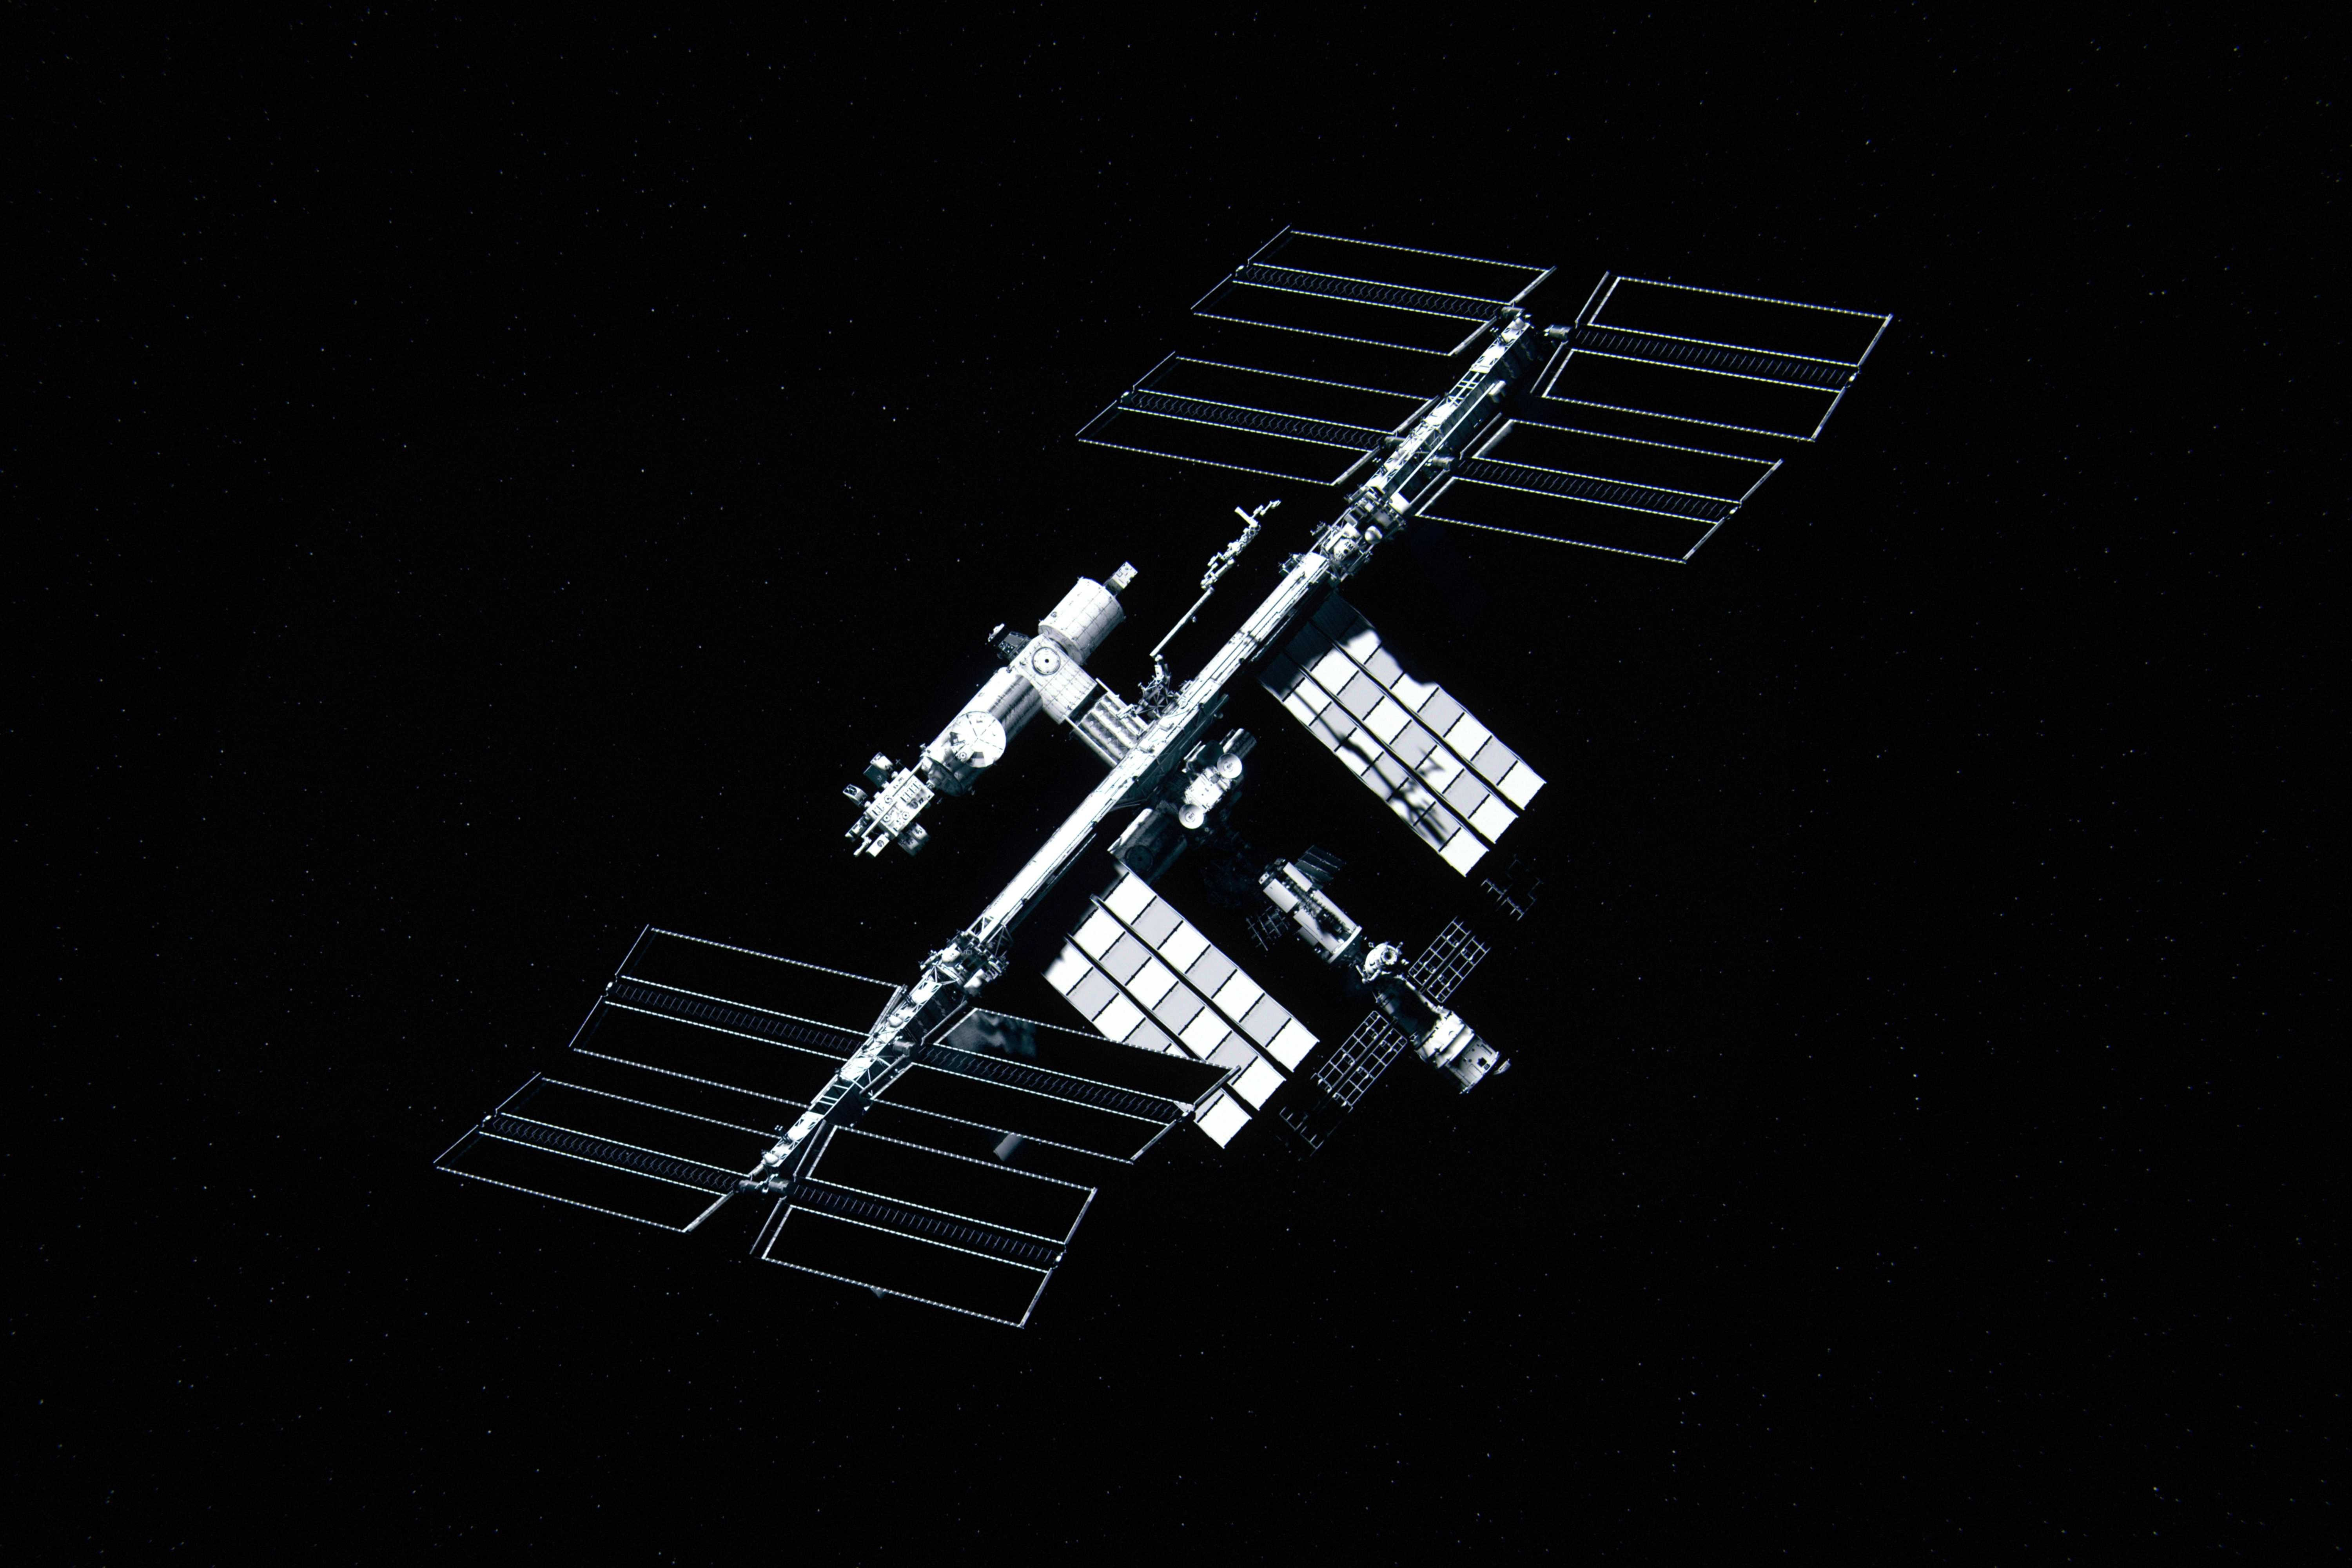
\includegraphics[height=3cm]{ISS}
    \end{center}


    \section{Die Konsole}\label{sec:die-konsole}
    \begin{exampleblock}{Fun Fact}
        \href{https://www.extremetech.com/extreme/155392-international-space-station-switches-from-windows-to-linux-for-improved-reliability}{Die ISS läuft seit 2013 auf Linux.}
    \end{exampleblock}
\end{frame}

\begin{frame}{Die "Wurzel"}

    \begin{quote}
        Die Wurzel (/), auch "root" genannt, ist der Ursprung des Dateisystems.
    \end{quote}
    \pause

    \begin{itemize}
        \item Die Wurzel ist ähnlich zum "C:\textbackslash"-Pfad in Windows\pause
        \item In "/home" leben alle Nutzer und ihre Daten\pause
        \item Dateisystem beginnt hier
    \end{itemize}

\end{frame}

\begin{frame}{Das Dateisystem}
    \subsection{Dateisystem}\label{subsec:dateisystem}

    \begin{quote}
        Alles in Linux ist eine Datei!?
    \end{quote}


    \begin{itemize}
        \item<2-> Konfigurationen (/etc)
        \item<3-> Commands (/bin)
        \item<4-> Geräte (/dev)
        \item<5-> Speichermedien (/media /mnt)
    \end{itemize}

    \vspace{0.5cm}
    \begin{exampleblock}{Fun Fact}<1->
        Dateien mit Punkt am Anfang (.bashrc .git) werden im Explorer standardmäßig versteckt.
    \end{exampleblock}
\end{frame}

\begin{frame}{Die Shell}
    \subsection{Die Shell}\label{subsec:die-shell}

    Die Shell ermöglicht direkten Zugriff auf das Betriebssystem.
    \pause

    \begin{itemize}
        \item Das mächtigste Werkzeug in Linux\pause
        \item Navigation durch das Dateisystem\pause
        \item Ausführen von System-Befehlen\pause
        \item Anzeige von Informationen
    \end{itemize}
    \pause

    \vspace{0.5cm}
    
\includegraphics[width=3cm]{plasma-konsole}
    \pause

    \vspace{0.5cm}
    \begin{alertblock}{Aufgabe}
        Öffne die Konsole und führe "whoami" aus.
    \end{alertblock}

\end{frame}

\begin{frame}{Befehle}
    \subsection{Befehle}\label{subsec:befehle}

    Ein Befehl besteht aus bis zu drei Teilen:
    \pause

    \begin{enumerate}
        \item Befehlsname\pause
        \item Optionen\pause
        \item Argumente
    \end{enumerate}
    \pause

    \vspace{0.5cm}
    \begin{exampleblock}{Beispiel}
        \$ ls -la /home/Nutzer/Dokumente
    \end{exampleblock}
    \pause

    \vspace{0.5cm}
    \begin{alertblock}{Aufgabe}
        Probiere diesen Befehl mit und ohne den Optionen bzw Argumenten.
    \end{alertblock}

\end{frame}

\begin{frame}{Navigation}
    \subsection{Navigation}\label{subsec:navigation}

    Wie navigiere ich durch das Dateisystem?
    \pause

    \textrightarrow "cd" wechselt den aktuellen Ordner
    \pause

    \begin{itemize}
        \item[\$] cd Ordnername\pause
        \item[\$] cd ..\pause
        \item[\$] cd
    \end{itemize}
    \pause

    \vspace{0.5cm}
    \begin{alertblock}{Aufgabe}
        Navigiere zum Ordner mit den Kurs-Dokumenten.
    \end{alertblock}
    \pause

    Platzhalter bei Befehlen:

    \begin{itemize}
        \item \textasciitilde\space für das Nutzer-Verzeichnis\pause
        \item . für den aktuellen Ordner\pause
        \item .. für den Überordner
    \end{itemize}

\end{frame}

\begin{frame}{Befehlshilfe}
    \subsection{Befehlshilfe}\label{subsec:befehlshilfe}

    Hilfe ich kenne diesen Befehl nicht!
    \pause

    \textrightarrow Zur Hilfe für unbekannte Befehle gibt es "man".
    \pause

    \vspace{0.5cm}
    \begin{alertblock}{Aufgabe}
        Ausprobieren:

        \begin{itemize}
            \item[\$] man man\pause
            \item[\$] man ls\pause
            \item[\$] man
        \end{itemize}
    \end{alertblock}
    \pause

    Wie komme ich da jetzt raus?
    \pause

    \textrightarrow Q drücken

\end{frame}

\begin{frame}{Textbearbeitung}
    \subsection{Textbearbeitung}\label{subsec:textbearbeitung}

    "nano" ist ein CLI-Programm zum Bearbeiten und Erstellen von Dateien.
    \pause

    \begin{itemize}
        \item CTRL + X zum Beenden\pause
        \item CTRL + O zum Speichern\pause
        \item CTRL + C zum Abbrechen des Speicherprozesses
    \end{itemize}
    \pause

    \vspace{0.5cm}
    \begin{alertblock}{Aufgabe}
        \begin{itemize}
            \item Erstelle eine Datei mit nano\pause
            \item[\$] nano test.txt
        \end{itemize}
    \end{alertblock}

\end{frame}

\begin{frame}{Dateien}
    \subsection{Dateien}\label{subsec:dateien}

    Umgang mit Dateien:
    \pause

    \begin{itemize}
        \item Bearbeiten: \$ nano datei.txt\pause
        \item Inhalt: \$ cat datei.txt\pause
        \item Entfernen: \$ rm datei.txt\pause
        \item Kopieren: \$ cp datei.txt neu.txt\pause
        \item Verschieben: \$ mv datei.txt neu.txt
    \end{itemize}
    \pause

    \vspace{0.5cm}
    \begin{exampleblock}{Tipp}
        Der "man"-Befehl kann beim Verständnis helfen.
    \end{exampleblock}

\end{frame}

\begin{frame}{Dateien - Übung}
    \subsubsection{Übung}\label{subsubsec:übung}

    \begin{alertblock}{Aufgaben}
        \begin{enumerate}
            \item Kannst du die Datei ".bashrc" finden?\pause
            \item Wann wurde die Datei zuletzt verändert?\pause
            \item Kopiere die Test-Datei in den Benutzerordner.\pause
            \item Benenne die Datei in "Ich-Kann-Bash" um.\pause
            \item Entferne die alte Datei.
        \end{enumerate}
    \end{alertblock}
    \pause

    \vspace{0.5cm}
    \begin{alertblock}{Extra}
        Informiere dich mithilfe von "man apt" über den APT-Befehl
    \end{alertblock}

\end{frame}

\begin{frame}{APT}
    \subsection{APT}\label{subsec:apt}

    APT ist der wichtigste Paket-Manager auf Debian/Ubuntu Systemen.
    \pause

    \textrightarrow Über shell steuerbar.
    \pause

    \begin{itemize}
        \item[\$] man apt\pause
        \item[\$] apt list \textminus\textminus installed\pause
        \item[\$] apt update\pause
        \item[\$] apt upgrade\pause
        \item[\$] apt install Programm\pause
        \item[\$] apt remove Programm
    \end{itemize}

\end{frame}

\begin{frame}{Sudo}
    \subsection{Sudo}\label{subsec:sudo}

    \begin{quote}
        Wie sagen wir, wenn wir höflich um Erlaubnis fragen?
    \end{quote}
    \pause

    \textrightarrow Richtig! "sudo"
    \pause

    \begin{itemize}
        \item Superuser do!\pause
        \item Lässt Admin-Befehle zu\pause
        \item Zum Schutz des "normalen" Nutzers\pause
        \item Mit Passwort-Eingabe verbunden\pause
        \item Steht direkt vor dem eigentlichen Befehl
    \end{itemize}
    \pause

    \vspace{0.5cm}
    \begin{exampleblock}{Beispiel}
        \begin{itemize}
            \item[\$] sudo apt install firefox
        \end{itemize}
    \end{exampleblock}

\end{frame}

\begin{frame}{Sudo}
    \begin{alertblock}{Aufgabe}
        Erledige diese Dinge mit der Shell:
        \begin{enumerate}
            \item<2-> Installiere "pdfpc"
            \item<3-> Entferne "okular"
            \item<4-> Aktualisiere dein System
        \end{enumerate}
    \end{alertblock}

    \vspace{0.5cm}
    \begin{exampleblock}{Fun Fact}<1->
        96,3\% des Internets läuft auf Linux-Servern
    \end{exampleblock}
\end{frame}

\begin{frame}{CLI Programme}
    \subsection{CLI Programme}\label{subsec:cli-programme}

    \begin{alertblock}{Aufgabe}
        Präsentiere PDFs von der Konsole aus:
        \begin{itemize}
            \item[\$] pdfpc präsentation.pdf\pause
            \item "TAB" zur Übersicht\pause
            \item "1,2,3,4" zum Modus wechseln\pause
            \item "CTRL + Q" zum Beenden
        \end{itemize}
    \end{alertblock}
    \pause

    Weitere CLI-Programme: nano, vim, man, htop ...

\end{frame}
